% !TEX root = hazelnut-dynamics.tex
%% \newcommand{\examplesSec}{Live Functional Programming in Hazel, By Example}
%% \newcommand{\examplesSec}{Live Programming in \HazelnutLive, By Example}
\newcommand{\examplesSec}{\HazelnutLive, By Example}
\section{\protect\examplesSec} % don't like the all-caps thing that the template does, so protecting it from that
\label{sec:examples}

\newcommand{\overviewExample}[2]{\paragraph{Example {#1}: {#2}}}

We introduce \HazelnutLive{} in this section using several examples,
demonstrating how running incomplete programs---with missing expressions and/or
type-inconsistent expressions---can be useful.
%
We will also demonstrate how running even complete programs with subexpressions
marked as holes may be useful in debugging.

\HazelnutLive{} programs are written in OCaml \cite{leroy03:_ocaml}, using the
alternative Reason syntax \cite{reason-what} extended to support holes.
%
As shown in \autoref{fig:grades-example}, a \HazelnutLive{} notebook is a
literate program \cite{knuth1984literate}: rich text comments appear at the top
level and code appears within cells embedded into these comments.
%
The reader is encouraged to work through these examples in our prototype
implementation or watch video demonstrations, both available in
\suppMaterials{}.\footnote{
%
The programs in this section are written using minor syntactic conveniences that
are not currently supported in our implementation.
%
For example, the implementation of recursive types in our current implementation
requires explicit \texttt{fold} and \texttt{unfold} expressions; these can be
inferred in standard ways (by pairing them with constructors and deconstructors
for algebraic datatypes) in future work.
%
More details about other minor syntactic differences are described in
\suppMaterials{}.
%
}


\subsection{Live Programming with Incomplete Expressions}

The process of writing new program fragments includes many states in which the
program under construction is, by definition, incomplete.
%
It is natural for a programmer to ``jump back and forth'' between different
places in the program, iteratively and alternately developing the missing
pieces.
%
The primary benefit of our approach is that such programs can be evaluated in
order to provide useful feedback during this editing workflow.

% !TEX root = hazelnut-dynamics.tex

\begin{figure}[t]
\begin{subfigure}[t]{\textwidth}
\centering
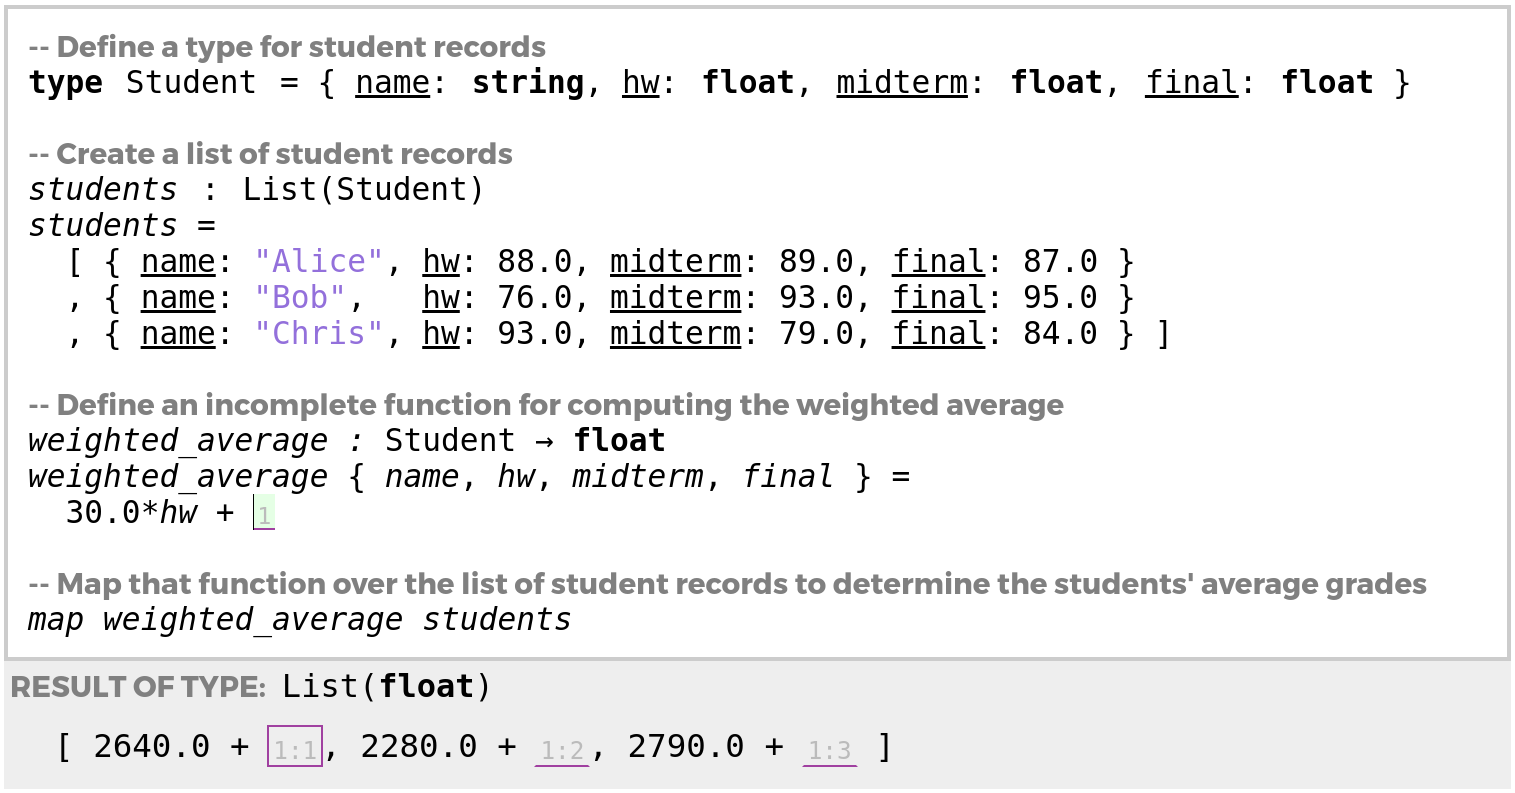
\includegraphics[width=0.8\textwidth,interpolate=false]{images/grades-cell-mockup.png}
\vspace{-3px}
\caption{Evaluating an incomplete functional program past the first hole}
\label{fig:grades-cell-mockup}
\end{subfigure}

\vspace{10px}

\begin{subfigure}[t]{\textwidth}
\centering
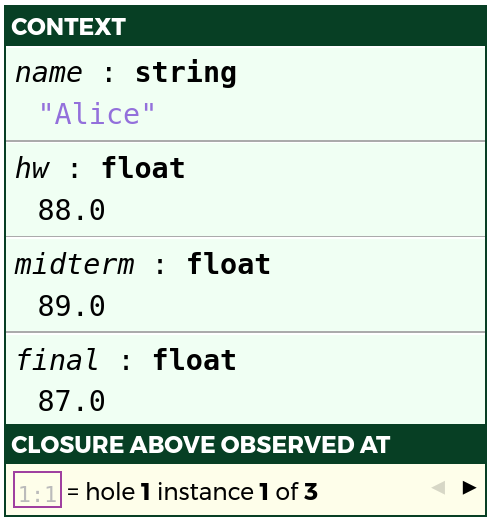
\includegraphics[width=0.29\textwidth,interpolate=false,valign=c]{images/grades-sidebar-1.png}
~${}^\blacktriangleright$
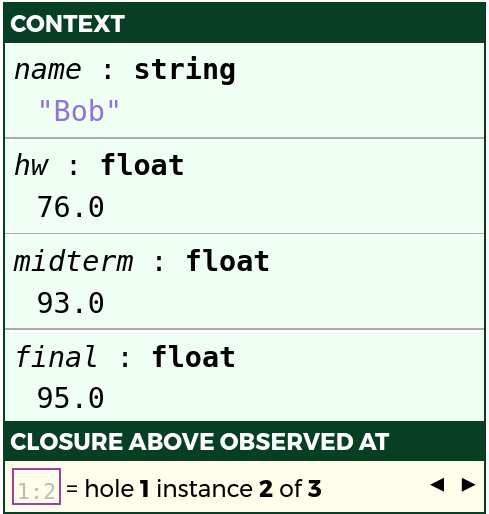
\includegraphics[width=0.29\textwidth,interpolate=false,valign=c]{images/grades-sidebar-2.png}
~${}^\blacktriangleright$
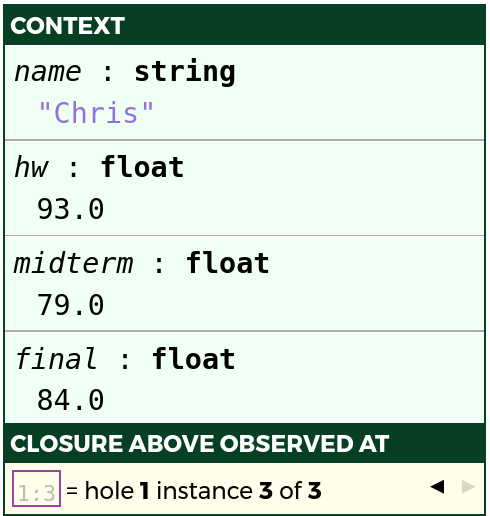
\includegraphics[width=0.29\textwidth,interpolate=false,valign=c]{images/grades-sidebar-3.png}
\caption{The live context inspector communicates relevant static \emph{and} dynamic information about variables in scope.}
\label{fig:grades-sidebar}
\end{subfigure}
% %% TODO once the code above is removed, scale up the screenshots
% 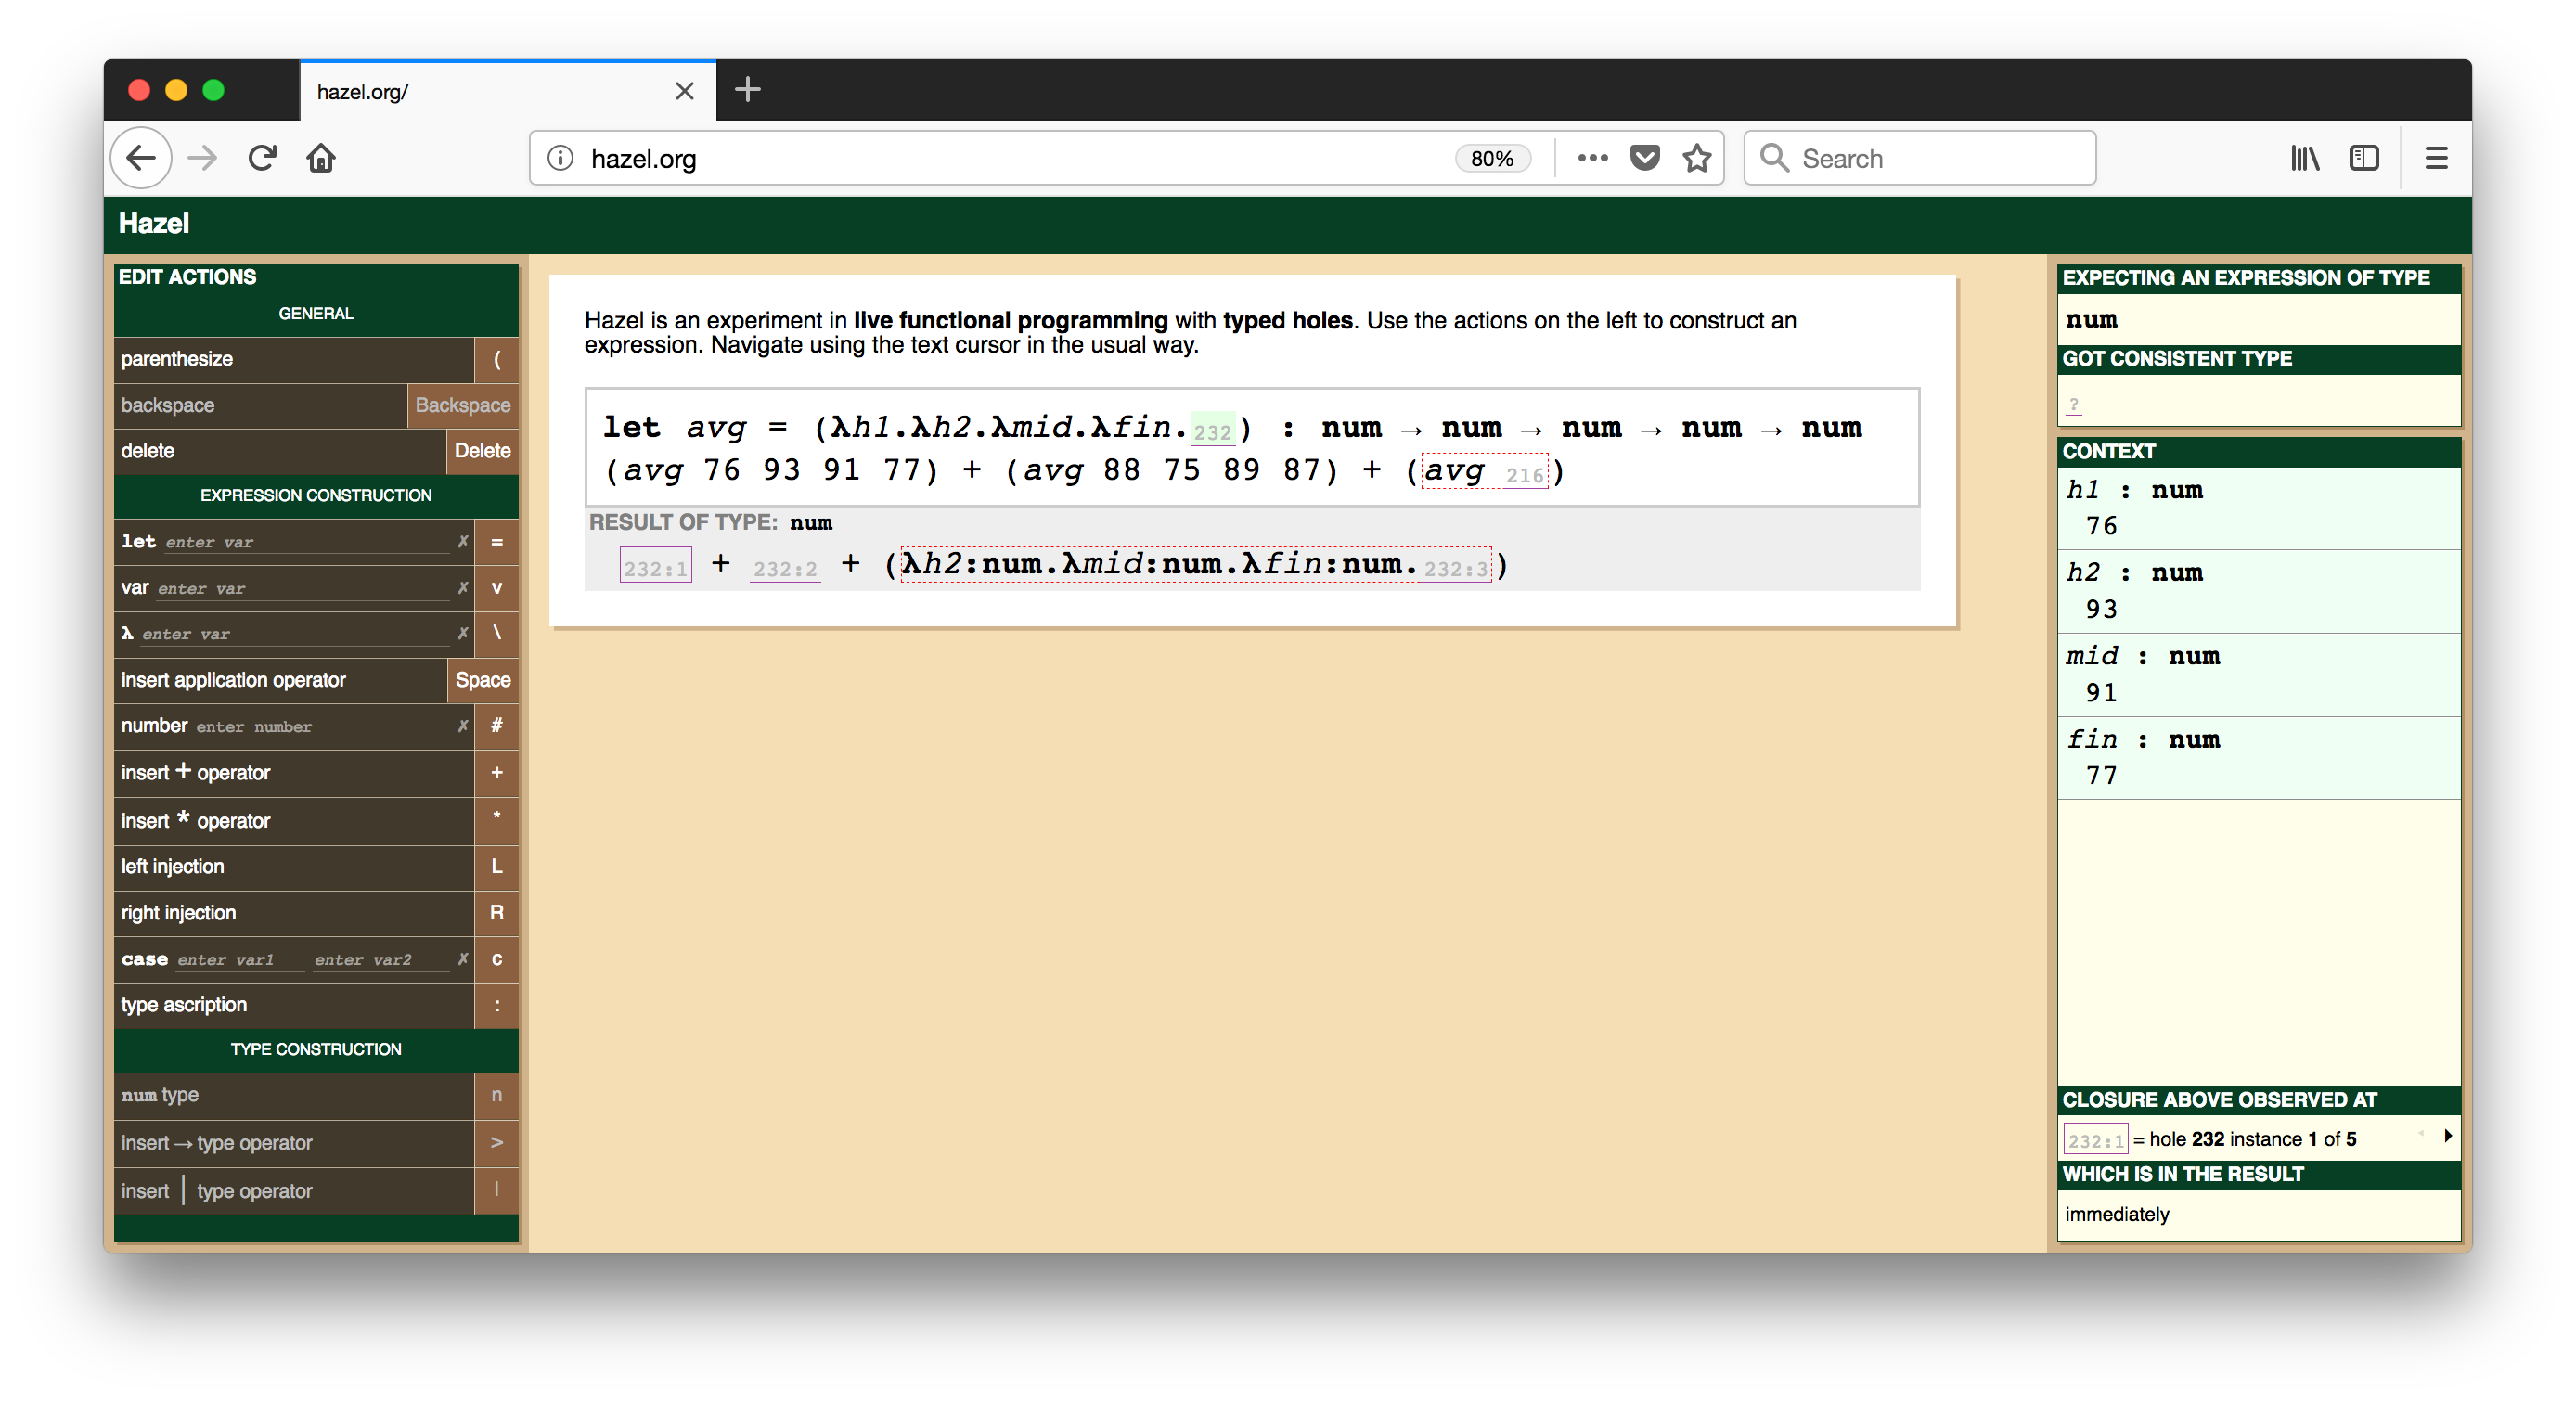
\includegraphics[scale=0.20]{images/hazel-placeholder-0.png}

% \rkc{Draw arrows and captions on the top figure to show how to get
% to the bottom figure.
% ser navigates to hole a, types + to create a plus, types * to create a
% multiplication, types \#10 to create 10, types vh1 to create variable use.}

% 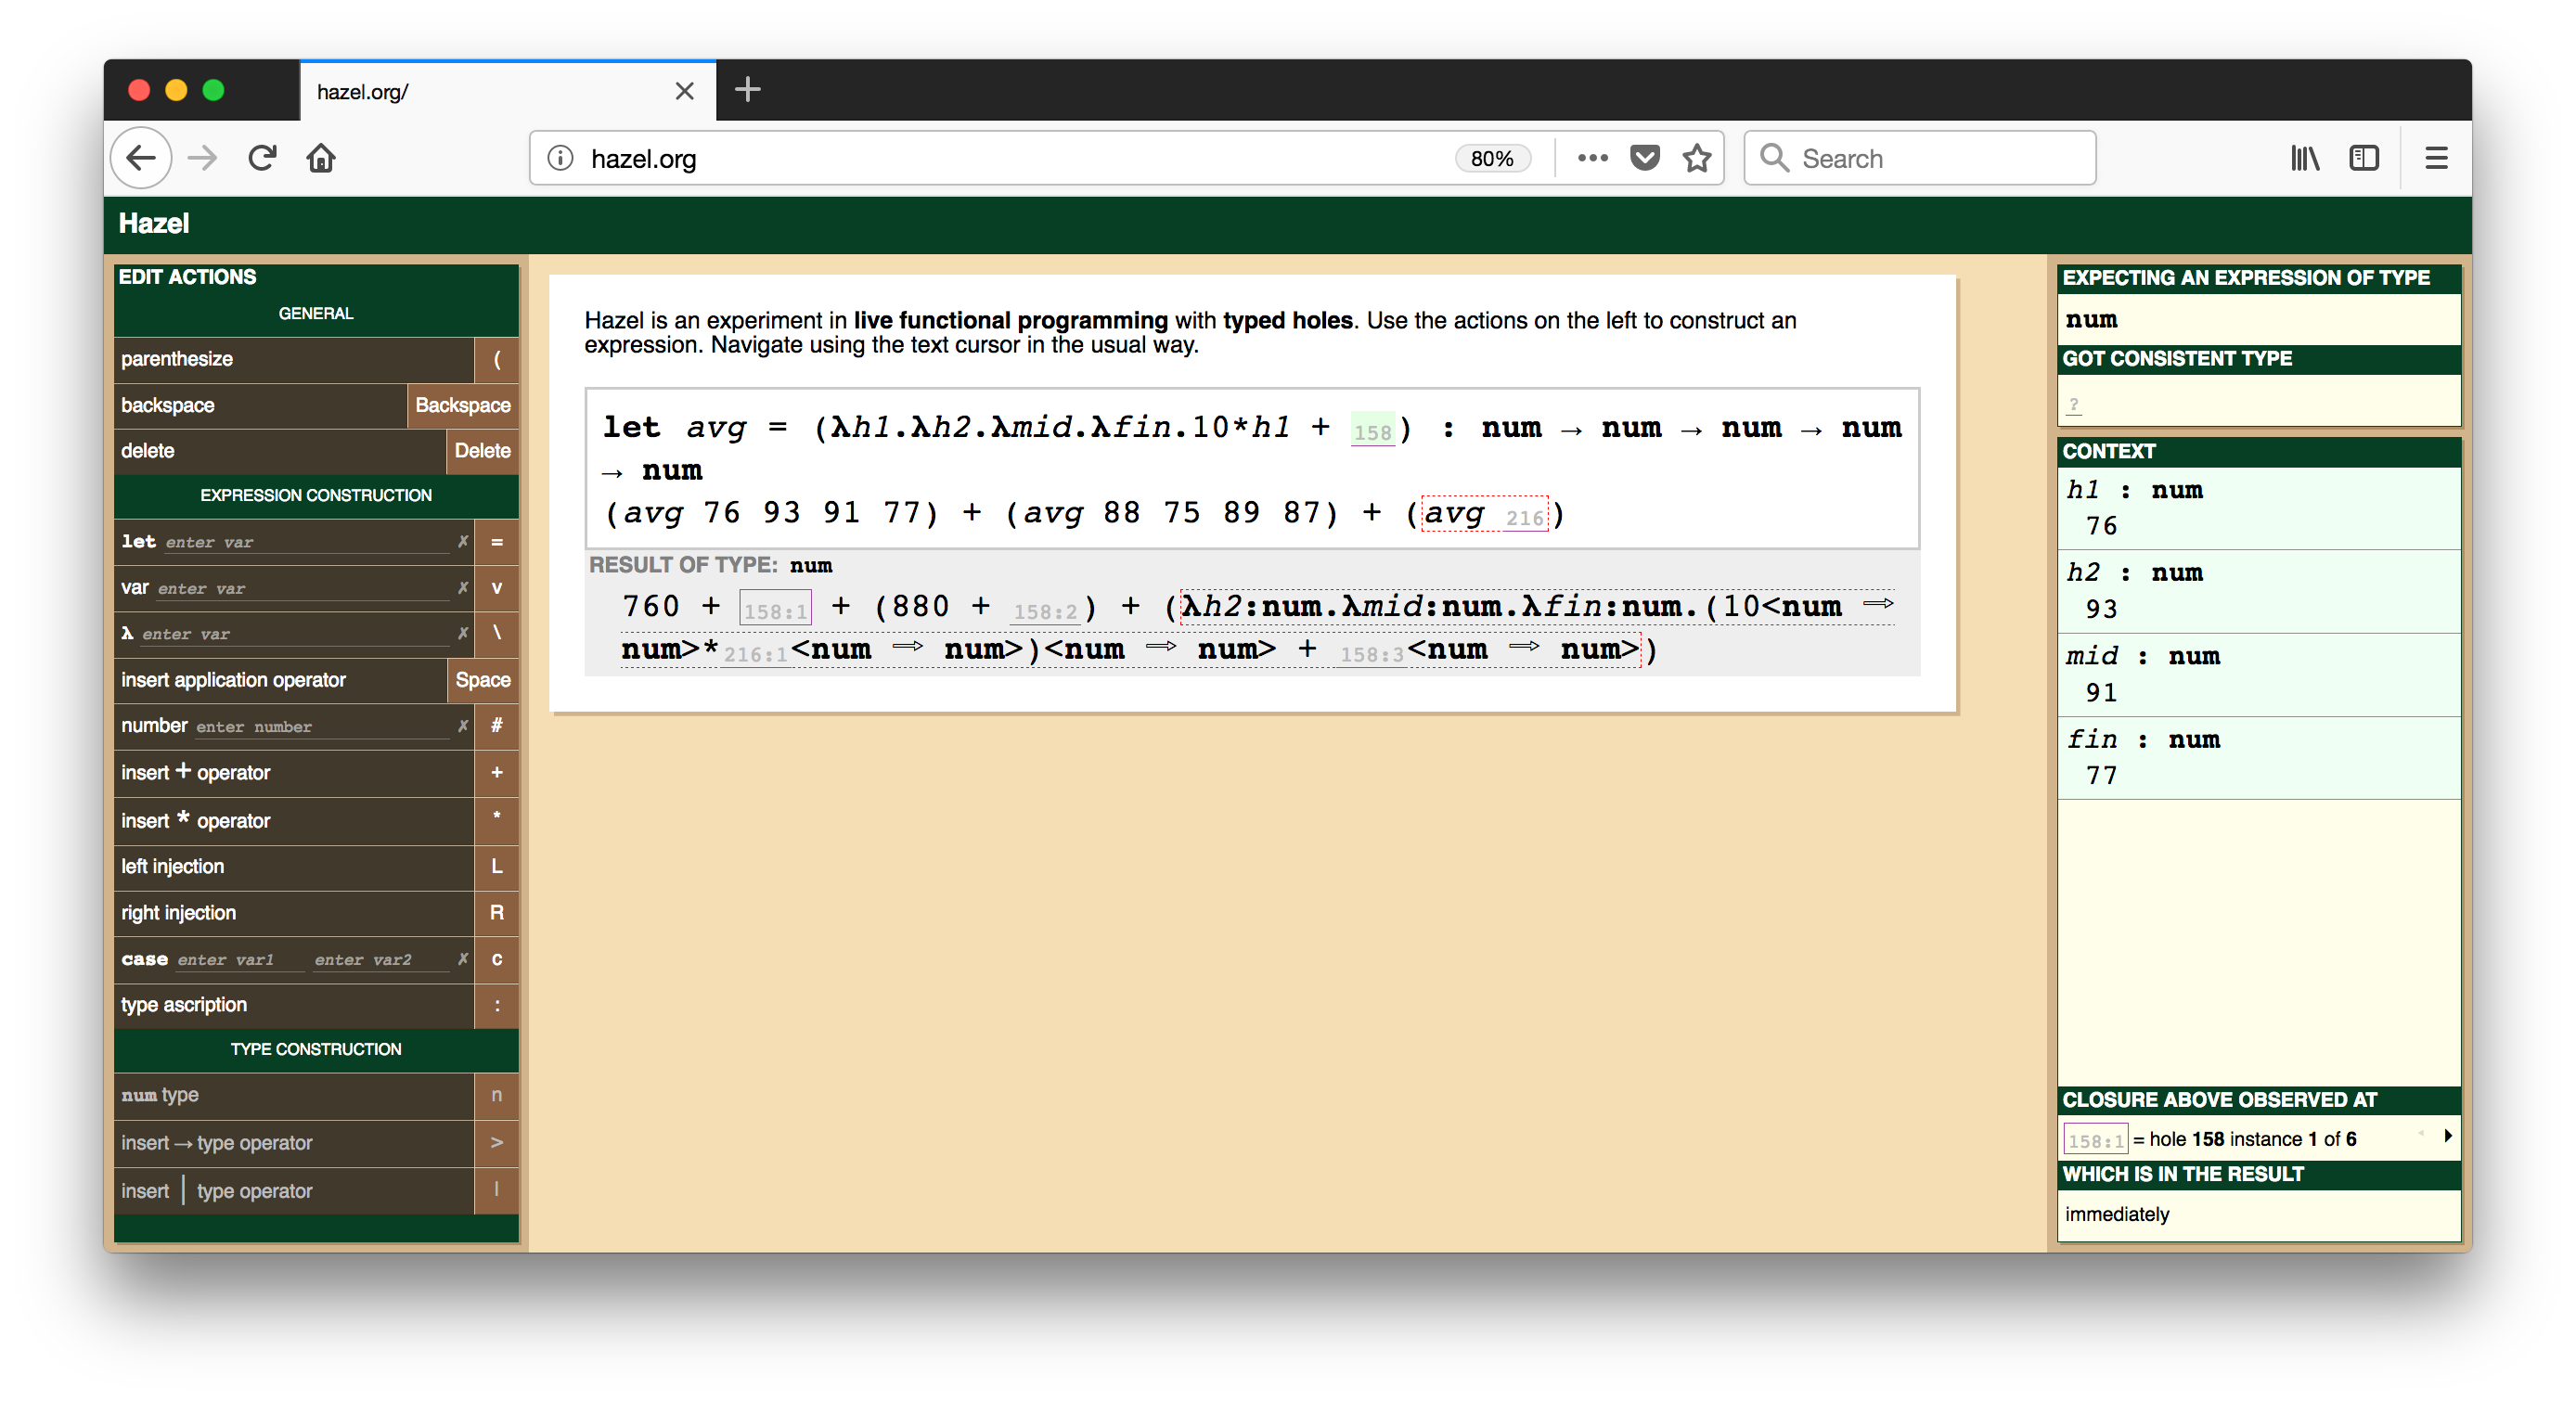
\includegraphics[scale=0.20]{images/hazel-placeholder-1a.png}
\vspace{3px}

\caption{Example 1: Grades}
\label{fig:grades-example}
\vspace{-5px}
\end{figure}


Consider a teacher who is in the midst of developing a \HazelnutLive{} notebook
(depicted in \autoref{fig:grades-example}) to compute final student grades at
the end of a term.
%
In the first cell in \autoref{fig:grades-example}, the teacher defines a record
type, \li{student_data}, for each student's course data.
%
In our simplified example, this includes the student's name, of type
\li{string}, and five grades, each of type \li{float}.

\overviewExample{1}{Computing Weighted Averages}
%
The teacher begins writing a \li{weighted_average} function that will
compute a weighted average, of type \li{float}, for each \li{student_data}
record.
%
The body of \li{weighted_average} is not yet written---marked with the
\emph{empty hole} on line \rkc{XXX}--- but the teacher jumps ahead to map the
function over the \li{grades} list.

\begin{lstlisting}
let weighted_average(g: student_data) =
  ??;

let weighted_averages = List.map weighted_average grades;
\end{lstlisting}

\noindent
%
\HazelnutLive{} evaluates this incomplete program, showing its
\emph{indeterminate} result in the sidebar on the right half of
\autoref{fig:grades-example}; this value is a list whose length is the same as
\li{grades}, where each element is the (indeterminate) result of evaluating the
hole expression inside \li{weighted_average}.
%
Notice that the hole on line \rkc{XXX} is assigned a unique static identifier
(\ie{}~\li{a}) and that the indeterminate results it produces are assigned
corresponding unique dynamic identifiers (\ie{}~\li{a.1}, \li{a.2}, etc.).
%
In contrast, the typical ad-hoc approach to simulating hole expressions, namely,
using placeholder expressions like \li{raise "Not yet implemented."}, would halt
the program as soon it is evaluated (in this case, inside the definition of
\li{List.map} when the function is applied to the first element of \li{grades}.
%
By ``evaluating around'' the hole in \HazelnutLive{}, the programmer can at
least see that the resulting expression does indeed evaluate to a list with the
correct number of (indeterminate) values.

Now the teacher returns to \li{weighted_average} to work on the missing
expression, with the goal of computing a weighted sum of each of a student's
grades.
%
The teacher uses a \HazelnutLive{} edit action to create a sum expression,
filling in the first summand by weighting the \li{hw1} score to account for 10\%
of the weighted average; the rest of the computation is a new hole expression
(\li{??_b}), yet to be filled in.

\begin{lstlisting}
let weighted_average(g: student_data) =
  (10.0 *. g.hw1) +. ??_b;
\end{lstlisting}

\noindent
%
\HazelnutLive{} immediately runs this incomplete program, displaying the updated
list of indeterminate expressions \li{[760.0 + ??_b.1, 880.0 + ??_b.2, ...]}.
%
Right away, the teacher recognizes that the values are too large; they should be
at most \li{100.0}.
%
The teacher realizes that representing percentage points as \li{float}s requires
that the constant on line \rkc{XXX} ought to be \li{0.10} instead.
%
Because of this live feedback, the teacher corrects this error right away and
avoids making similar programming errors in the rest of the calculation.
%
The teacher continues to build the rest of the arithmetic expression until it is
complete (there are no longer any expression holes), and the result of
immediately running the finished program shows that each of values in the final
result list is in the range \li{0.0} to \li{100.0}.

\overviewExample{2}{Assigning Letter Grades}
%
The teacher's next task is to map the weighted averages to the letter grades A
through F (we will consider only ``whole'' letter grades, for simplicity).
%
The \li{grade_cutoffs} record type describes the minimum cutoff for each of
these six possible grades.
%
Initially, each value in the \li{cutoffs} record is a hole.

\begin{lstlisting}
type grade_cutoffs =
  { a: float, b: float, c: float, d: float, f: float };

let cutoffs =
  { a = ??_a, b = ??_b, c = ??_c, d = ??_d, f = ??_f };
\end{lstlisting}

\noindent
%
%% initially all holes, because it will be different year-to-year based on the %
%data, differences in course difficulty, and to satisfy fairness criteria.
%
Before starting to fill in the cutoffs, the teacher jumps ahead to write a
function \li{letter_grade} that will make the connection between \li{cutoffs}
and \li{weighted_averages}.
%
Because she intends to look at the data to help select the cutoff values, the
teacher sorts the \li{weighted_averages} and then maps them to
\li{letter_grades}.

\begin{lstlisting}
let letter_grade(n: weighted_average) =
  if n >= cutoffs.a then "A" else
  if n >= cutoffs.b then "B" else
  if n >= cutoffs.c then "C" else
  if n >= cutoffs.d then "D" else
  if n >= cutoffs.f then "F" else "Incomplete";

let sorted_weighted_averages = List.sort weighted_averages;

let letter_grades = List.map letter_grade sorted_weighted_averages;
\end{lstlisting}

\noindent
%
When \HazelnutLive{} runs this program, the guard of the outermost conditional
(\li{n >= cutoffs.a} on line \rkc{XXX}), is indeterminate because \li{cutoffs.a}
is.
%
Therefore, each of the indeterminate expressions in \li{letter_grades} is the
entire expression body, albeit with different bindings for \li{n}.
%
Displaying such ``large'' indeterminate expressions can quickly consume all
available screen space, overwhelming the user with too much information.
%
\autoref{fig:XXX} shows how \HazelnutLive{} renders large indeterminate
expressions (\ie{}~anything other than ``small'' indeterminate value (a constant
or hole) or list of small values) simply as \li{..} to save space.
%
Hovering over this abbreviation (as shown in \autoref{fig:XXX} displays the full
indeterminate expression---as well as the evaluation environment that surrounds
it---as a tooltip.
%
\autoref{sec:discussion} discusses this and other user interface concerns when
trying to display useful live feedback without overwhelming the user.
%
These usability factors are beyond the scope of our work, which is to define
semantic foundations on which such user interfaces can be built.

To start deciding \li{cutoffs}, the teacher looks at the \li{weighted_averages}
sorted in descending order.
%
The data shows a natural gap between \li{92.2} and \li{89.5}.
%
So, she chooses to use \li{92.0} as the cutoff for A.
%
Resuming the computation from before, \HazelnutLive{} resolves the conditional
expressions for the first \rkc{XXX} indeterminate expressions, because each of
those \li{n} values was greater than \li{cutoffs.a}.
%
The remaining \rkc{XXX} expressions also proceeded to evaluate the first guard,
and are now indeterminate at the guard for the second conditional.

Before assigning other cutoff values, the teacher would like to get a sense of
whether this first choice is a good one.
%
She jumps ahead to to write a function that computes the distribution of letter
grades.

\begin{lstlisting}
let compute_distribution(list: list(float)) =
  let n = List.length letter_grades in
  List.map
    (\x -> (x, showPercentage (List.length (List.filter ((==) x) list)) /. n))
    ["A","B","C","D","F","Incomplete"];

let distribution = compute_distribution(letter_grades);
\end{lstlisting}

\noindent
%
Running \li{compute_distribution} shows that the percentage of As is
\rkc{XXX\%}, which is smaller than what the teacher would like;
the remaining percentages are all indeterminate.
%
Returning to the value of \li{sorted_data}, she sees a cluster around \li{89.0}
and then another gap between \li{88.2} and {85.5}.
%
So, the teacher adjusts \li{cutoffs.a} to be \li{88.0}.
%
Because this edit is outside of a hole expression, \HazelnutLive{} discards the
previous execution state and reevaluates the entire program.
%
Existing techniques for incremental computation~\cite{XXX,XXX}, however, could
be applied to seek opportunities for reuse even when non-hole expressions are
modified.
%
Because the focus of work is on the novel implications of running programs with
holes, our calculus and implementation supports caching ``edit-and-resume'' only
for the novel situation in which evaluation proceeds around holes.
%
After re-evaluation, the percentage of As becomes \rkc{XXX\%}, which better
matches the teacher's intention.

In this fashion, the teacher continues down the list of sorted averages,
determining appropriate values for each cutoff.
%
Whenever the teacher is only filling in the ``next'' cutoff, the computation
from before can simply be resumed.
%
Overall, throughout the workflow described in these two examples, the programmer
can continue to evaluate the program, and receive meaningful feedback, while
going back and forth between different pieces under development.


%% \subsection{Live Programming with Type Errors}
\subsection{Live Programming with Static Type Errors}

In the previous section, we described example programs that were incomplete
because of \emph{missing} expressions.
%
Next, we describe example programs that are incomplete because of
\emph{type-inconsistent} expressions.
%
For example, consider the following two definitions.

\begin{lstlisting}
let bad_bool : bool = ?? 0 ??_bad_bool;

let bad_int : int = 1 + ?? true ??_bad_int_second_argument;
\end{lstlisting}

\noindent
%
These two definitions are ill-typed under standard typing disciplines.
%
In contrast, \citet{popl-paper} present a bidirectional type system that assigns
types to both, by wrapping type-inconsistent expressions (\li{0} on line
\rkc{XXX} and \li{true} on line \rkc{XXX} above) in \emph{non-empty} holes.
%
Non-empty holes prevent local type inconsistencies from polluting the rest of
the program surrounding it, which may or may not itself contain additional
inconsistencies.

Understanding and debugging static type errors is notoriously difficult,
particularly for novices.
%
A variety of approaches have been
proposed~\cite{Seminal,ChenErwig2014,Pavlinovic2015,sherrloc} to better localize
and explain type errors.
%
One of these approaches~\cite{Seidel2016} proposes to generate a dynamic witness
that demonstrates a run-time failure, and then displays a compressed execution
trace to the user as a graph.
%
In \HazelnutLive{}, we can run programs with type errors (\ie{}, programs with
non-empty holes) as far as possible, in particular, until they
would go wrong.
%
Thus, our operational semantics provides a similar benefit to the approach of
\citet{Seidel2016}.

\overviewExample{3}{Sum List}
%
Consider the following buggy program (observed during an undergraduate
functional programming course~\cite{Seidel2016}) that attempts to sum a list
integers.
%
The error is that the base case produces a list rather than an integer.

\begin{lstlisting}
sumList : list(int) -> int
sumList [] = ?[]?
sumList (n:ns) = n + sumList ns
\end{lstlisting}

\noindent
%
Because the list expression on line 2 does not have type \li{int} as required,
it is wrapped in a (non-empty) hole by the bidirectional type
checker~\cite{popl-paper}.
%
Rather than trying to debug the error based on the static error, the programmer
may wish to trying running the function anyway by calling, say, \li{sumList(2)}.
%
\HazelnutLive{} runs and produces the indeterminate expression \li{3 + ?[]?}.
%
By observing that the hole expression is being added to the integer \li{3}, he
realizes that it needs to be an integer, specifically, \li{0}.
%
Compared to the trace displayed by \citet{Seidel2016}, the indeterminate result
produced by \HazelnutLive{} is ``flattened'' because the expression \li{1 + 2}
successfully proceeded to evaluate despite the error elsewhere.


%% TODO fold error from Erwig paper.
%% %
%% see that final call on stack does have the right answer, but
%% it's wrapped in a singleton list when the expected type is not
%% a list.
%% %
%% fix is to remove the list, the rest of the computation remains
%% the same, but b/c they were all wrapped in holes, need to re-run.
%% %
%% (add some mechanism for type-consistent non-empty-holes...)

\overviewExample{4}{Stutter}
%
Consider the following function which attempts to produce a
list where every element is repeated twice (borrowed from \citet{Osera2015}).
%
The combiner function to \li{List.foldr} needs to produce a \li{list(int)}, but
it produces a \li{list(list(int)} instead.

\begin{lstlisting}
stutter : list(int) -> list(int)
stutter xs = List.foldr (\x acc -> ?[x,x]? : acc) [] xs
\end{lstlisting}

\noindent
%
The bidirectional type checker of \citet{popl-paper} wraps the expression
\li{[x,x]} inside a non-empty hole.
%
%% The editor has a choice about which expression to ``blame'' for the error; the
%% entire application that forms the body of the lambda is analyzed against the
%% return type \li{list(int)}, so that is a reasonable choice for the editor to
%% make; another would be to assume that the arguments \li{[x,x]} and \li{acc} are
%% both as intended and that only the function \li{(:)} is type-consistent.
%% %
%% Although one could imagine a setting in which a user would perform this
%% reasoning, let's assume the simplest approach for marking consistencies that
%% wraps the entire application.
%
Running this on \li{stutter [1,2,3]} produces the indeterminate result

\begin{lstlisting}
?  [1,1] : (? [2,2] : (? [[3:3]] ?) ?) ?,
\end{lstlisting}

\noindent
%
which shows the unfolding of \li{List.foldr}.
%
We refer to nested indeterminate computations like this as \rkc{\emph{hole
environment traces} or \emph{hole environment trees}}.
%
The result of the innermost indeterminate expression is \li{[[3,3]]}.
%
The user realizes that there are too many levels of nesting, so
he replaces the \li{(:)} with \li{(@)}, which addresses the type inconsistency
and, when reevaluated, produces the desired result.


\subsection{Live Programming with Gradual Type Errors}

An alternative to marking type-inconsistent expressions as sources of error
(with non-empty holes) is to use \emph{gradual types}~(\eg{}~\cite{XXX,XXX,XXX})
to sidestep the choice of a assigning single static type, instead deferring to
dynamic casts.
%
\HazelnutLive{} inherits the notion of \emph{type holes} from
\citet{popl-paper}, which serves a similar static purpose as the unknown type in
gradual type systems.

\overviewExample{5}{Dynamically Typed Negation}

Consider the \li{negate} function (adapted from \cite{ChughPOPL2012}), which
does not have a conventional static type (without using expression holes),
because the argument \li{x} is used at type \li{int} on line \rkc{XXX} and
function type on line \rkc{XXX}.
%
Therefore, the declared type of \li{x} is the hole type \li{??}, which allows
\li{x} to be used at conflicting types by expanding each use with \emph{casts}
that ensure the safety of each dynamic use.
%
The return type also uses the hole type \li{??}.

\begin{lstlisting}
negate : bool -> ?? -> ??
negate b x =
  if b
    then 0 - x     // expanded to: (0 - (x<?? => int>))<int => ??>
    else not x     // expanded to: (not (x<?? => bool>))<bool => ??>

(negate false 1) + 2 + 3 + (negate true 4)
\end{lstlisting}

\noindent
%
As in prior gradually typed languages~\cite{XXX},
evaluating the expression \li{negate true 1} on line \rkc{XXX} leads to
\li{(not (1<int => ??><?? => bool>))<bool => ??>}, where the inner casts
lead to the \emph{cast error} \li{1<?? =/=> bool>} because \li{1} cannot be
safely treated as having type \li{bool}.
%
Unlike in prior gradually typed languages, however, \HazelnutLive{} evaluates
around the cast error, making progress on the \li{2 + 3 + negate false 4}
expression that surrounds the error; the final indeterminate result is
\li{(not (1<?? =/=> bool>))<bool => ??> + 1}.
%
Just like it is useful for static type checkers to report multiple errors, our
approach allows us to report multiple dynamic cast errors, and otherwise make
progress on expressions that do not depend on failed casts.
%
This approach can be incorporated into existing gradually typed languages.


\rkc{STOPPING HERE FOR NOW}

\subsection{Live Programming for Debugging}

\overviewExample{6}{\rkc{...}}

\rkc{breakpoints, understanding input/output behavior}

\parasection{Example 6: Quicksort}

\begin{lstlisting}
quicksort : list('a) -> list('a)
quicksort [] = []
quicksort (x:xs) =
  let (left, right) = span ((>) x) xs in
  ??
\end{lstlisting}

programmer has some intended relationship between names and values they bind.
%
live results show that left has larger elements and right has smaller.
%
right away, can see that need to change filter predicate. (alternatively, the
names could have been swapped, but that order of names was the natural way
to think about it.)
%
but next, still see that right has some smaller elements.
%
should pick partition instead of span.

\begin{lstlisting}
quicksort : list('a) -> list('a)
quicksort [] = []
quicksort (x:xs) =
  let (left, right) = partition ((<) x) xs in
  let (left', right') = (quicksort left, quicksort right) in
  ? (left' @ [x] @ right) ?
\end{lstlisting}

now, put the lists back together.
%
doesn't do what is expected.
%
live feedback shows right' is computed correctly, but ah, it's not being used
in the return list.
%
fix, and re-run, keeping the final expression in a hole.
%
can visualize that the nested appends are being built up correctly, and that the
result would be the correct list.
%
finalize the hole and resume. everything but the nested appends can be reused.
%
\emph{hole environment traces} or \emph{hole environment traces}

\paragraph{Recap}
%
In the above four subsections, respectively, we considered programs with:
%
(1) empty expression holes,
%
(2) non-empty expression holes for ill-typed expressions,
%
(3) type holes, and
%
(4) non-empty expression holes for well-typed expressions.
%
Next, we will formally describe the novel dynamic semantics of \HazelnutLive{}
that allows programs with combinations of these kinds of incompleteness to be
evaluated.
